\documentclass[a4paper,11pt]{article}

% Package to make citations superscrit with brackets
%\usepackage[super,square]{natbib}

\usepackage[style=apa]{biblatex}
\addbibresource{references.bib}

% Package to change margin size
\usepackage{anysize}
\marginsize{2cm}{2cm}{1cm}{2cm}
% Package to make headers
\usepackage{fancyhdr}
\setlength{\headheight}{13.6pt} % Fix for fancyhdr warning
\renewcommand{\headrulewidth}{0pt}
% Package for highligths
\usepackage{soul}
% Colors for the references links
\usepackage[dvipsnames]{xcolor}
% Package to link references
\usepackage{hyperref}
\hypersetup{
    colorlinks=true,
    linkcolor=black,
    citecolor=CadetBlue,
    filecolor=CadetBlue,      
    urlcolor=CadetBlue,
}
% Package for lorem ipsum
\usepackage{lipsum}
% Package for multicolumn
\usepackage{multicol}
% Package for removing paragraph identations
\usepackage{parskip}
\setlength\columnsep{18pt}
% Sets abstract
\renewenvironment{abstract}
 {\par\noindent\textbf{\abstractname}\ \ignorespaces\\}
 {\par\noindent\medskip}

\usepackage{graphicx}

\usepackage{amsmath}

\usepackage{caption}

\usepackage{amssymb}

\usepackage{tikz}

\usepackage{float}



\begin{document}

\begin{titlepage}
    \pagestyle{empty}
    \begin{center}
        % Logo
        
\includegraphics[width=0.25\textwidth]{isologo-utec.png} % Adjust path/size as needed
        \vspace{1cm}

        % Title
        {\LARGE\textbf{Modelo numérico de tiempos de impulso para optimización de trayectorias en misiones de interceptación orbital}}
        \vspace{1.5cm}

        % Authors
        {\large
            \textbf{Integrantes:} \\
            Camargo, Aldo: 202020023 \\
            Casquino, Daniel: 202110056 \\
            Vargas, Gabriel: 202310129 \\
            Whitty, Emma: 202310170 \\
            Zelaya, Jerusalén: 202220361 \\
        }
        \vspace{1cm}

        % Course
        {\large
            \textbf{Curso:} Métodos Numéricos
        }
        \vspace{0.5cm}

        % Teacher
        {\large
            \textbf{Docente:} Perez Cupe, Rosulo
        }
        \vspace{0.5cm}

        % Date
        {\large
            \textbf{Fecha de presentación:} 11 de mayo de 2025
        }
        \vfill

        {\large
            Universidad de Ingeniería y Tecnología (UTEC)
        }
    \end{center}
\end{titlepage}

% Makes header
\pagestyle{fancy}
\thispagestyle{empty}
\fancyhead[R]{\textit{Universidad de Ingeniería y Tecnología --- UTEC}}
\fancyhead[L]{}
% Makes footnotes with an asterisk
\renewcommand*{\thefootnote}{\fnsymbol{footnote}}

\begin{abstract}
    En el contexto de exploración espacial, la planificación de las trayectorias y
cambios de dirección requieren una cantidad considerable de apoyo terrestre. En
este contexto, surge el interés por minimizar los impulsos necesarios para
interceptar objetivos. Dados una nave perseguidora y dos objetos a interceptar,
(Xia et al., 2021) plantea una solución general para interceptar a los dos
objetos con un sólo impulso. Utilizando el método de Gibbs, se logra plantear
un sistema de ecuaciones no lineales de dos variables, el cual se puede
resolver numéricamente con el Método de Newton Raphson. Este documento busca
aplicar métodos numéricos para resolver casos particulares en MATLAB, así como
analizar la convergencia y compararla con otros métodos.
\end{abstract}

\noindent\textbf{Palabras clave:} intercepción orbital, método de Gibbs, método de Newton-Raphson, Porkchop plot, mecánica orbital, Two Body Model
\vspace{0.5cm}

{\color{gray}\hrule}
\medskip
\begin{multicols}{2}
    \renewcommand{\contentsname}{Índice}
    \tableofcontents
    \section{Introducción}

La exploración espacial ha avanzado significativamente gracias al desarrollo de tecnologías
que permiten ejecutar misiones más eficientes y de bajo costo. Sin embargo, la planificación de las trayectorias
y cambios de dirección siguen requiriendo una cantidad considerable de apoyo terrestre. En este contexto, surge el interés
por minimizar la cantidad de impulsos para llegar o interceptar a objetivos, una tarea importante en el mantenimiento de satélites
y exploración interplanetaria \parencite{ZHU20162177}.

El trabajo de Xia et al. (2021) propone un método numérico para resolver el problema de intercepción de dos objetivos
con un solo impulso, permitiendo posiciones de impulso e intercepción libres, tanto en órbitas elípticas como hiperbólicas \parencite{xia2021}.
Este enfoque reduce el problema original —de seis variables— a un sistema no lineal de solo dos variables independientes,
resuelto con el método de Newton-Raphson y estimaciones iniciales obtenidas mediante \textit{porkchop plots}.
Además, se extiende a modelos perturbados por el coeficiente J2 utilizando homotopía y corrección diferencial.

Estudios complementarios, como el de Duan y Liu (2020), exploran alternativas al clásico método de porkchop plots,
proponiendo un enfoque bidimensional más eficiente para determinar ventanas de lanzamiento, lo cual puede ser útil
en la etapa de estimación inicial de trayectorias \parencite{DUAN2020965}.

Por otro lado, el uso de propulsión eléctrica en satélites pequeños, como los CubeSats, ha abierto nuevas posibilidades para
misiones autónomas más complejas. Sistemas como los \textit{electrospray thrusters} o los \textit{gridded ion thrusters} ofrecen maniobras
precisas con menos consumo de combustible, lo cual refuerza la relevancia de modelos como el propuesto por Xia et al.\@ para planificar
trayectorias de forma óptima \parencite{oreilly2021}.

De forma complementaria, Zhu y Yan (2016) presentan un esquema de maniobra con dos impulsos tangenciales
en órbitas elípticas, que enfatiza la eficiencia de combustible bajo restricciones de tiempo y geometría, lo que sustenta
la importancia de estudiar intercepciones óptimas desde un punto de vista numérico \parencite{ZHU20162177}.
    \section{Objetivos}
\subsection{Objetivo General}
Crear un modelo computacional usando métodos numéricos que nos ayuden a resolver el problema de intersección de dos objetivos con un solo impulso. Se utilizará el método de Newton-Raphson y la matriz de Jacobiana para poder resolver el sistema de ecuaciones no lineales.
\subsection{Objetivos Específicos}
\begin{itemize}
    \item Utilizar el método numérico de Newton-Raphson utilizando una matriz jacobiana analítica para poder resolver el sistema de ecuaciones no lineales que describe el problema de intersección de dos objetos en un momento orbital.
    \item Evaluar el comportamiento del modelo en distintas condiciones iniciales como posiciones y velocidades.
    \item Analizar la precisión y eficiencia del modelo, evaluando la convergencia en distintos escenarios de intercepción. Comparando los resultados con los obtenidos en el artículo de referencia.
    \item Determinar cuales son los valores óptimos de impulso y del tiempo de aplicación, permitiéndonos interceptar el objetivo, considerando la trayectoria orbital establecida.
\end{itemize}

    \section{Justificación}

Resolver el problema de intersección de dos cuerpos en movimiento
con un sólo impulso es importante porque nos permite desarrollar
soluciones eficientes ante situaciones críticas donde se cuenta
con recursos limitados.

El uso y análisis de métodos numéricos permite comparar el desempeño de las distintas
estrategias de optimización, dando lugar a posibles mejoras con la elección de distintos
métodos. Esto contribuye al desarrollo de de modelos que trabajan con más objetivos, y por
ende reducen aún más el uso de combustible.
    \section{Marco Teórico}
\subsection{Definiciones}
\begin{itemize}
    \item \textbf{Nave perseguidora}: nave que realiza los impulsos y busca interceptar a los dos objetos.
\end{itemize}

\subsection{Conceptos}
El problema de interceptación de dos objetivos con un solo
impulso es un reto fundamental en la mecánica orbital, particularmente en las
misiones espaciales que requieren la optimización de maniobras para
minimizar el uso de combustible \parencite{Battin1999}.
\subsubsection{Interceptación Orbital}
La interceptación orbital es el proceso
mediante el cual una nave espacial ajusta su trayectoria para alcanzar
un objetivo en el espacio.
\subsubsection{Two-Body Model}
El modelo de dos cuerpos es un modelo simplificado en mecánica orbital
que describe el movimiento (elíptico) de dos cuerpos bajo la influencia
mutua de la gravedad, sin tener en cuenta otras fuerzas externas (como las
perturbaciones atmosféricas) \parencite{Cerf2013}.
\subsubsection{Impulso}
En astrodinámica, el impulso es un cambio abrupto en la
velocidad de una nave espacial, que altera su trayectoria orbital.
\subsubsection{Transferencia}
Las transferencias elípticas
son trayectorias cerradas en forma de elipse, mientras que las
transferencias hiperbólicas son trayectorias abiertas que permiten a
un objeto escapar de la atracción de un cuerpo central (como la
Tierra) \parencite{ZHU20162177}.
\subsubsection{Perturbación J2}
La perturbación J2 es el efecto causado por la
forma no esférica de la Tierra, que altera ligeramente las órbitas de
los objetos cercanos debido a la asimetría gravitacional de la Tierra
(concentrada en el ecuador).
%
\subsection{Métodos Numéricos}
\subsubsection{Gráfico Porkchop}
Este método se utiliza para visualizar las posibles combinaciones de
los tiempos de impulso $t_0$ y tiempos de intercepción $t_1$ que minimizan
el tiempo total de la misión o el uso de combustible \parencite{DUAN2020965}.

El gráfico de Porkchop calcula el coste asociado a cada combinación
de $t_0$ y $t_1$ mediante una fórmula de la forma:

\begin{equation}
    \begin{split}
        P(t_0, t_1) = \left| t_1 - t_0 - \frac{M_3(t_1) - M_3(t_0)}{n_3} \right| \\
        + \left| t_2 - t_0 - \frac{M_3(t_2) - M_3(t_0)}{n_3} \right|
    \end{split}
\end{equation}


\begin{itemize}
    \item $M_3(t)$: anomalía media en el tiempo $t$.
    \item $n_3$: movimiento medio de la órbita de la nave perseguidora.
    \item $t_2$: tiempo de intercepción con el segundo objetivo.
\end{itemize}

\begin{center}
    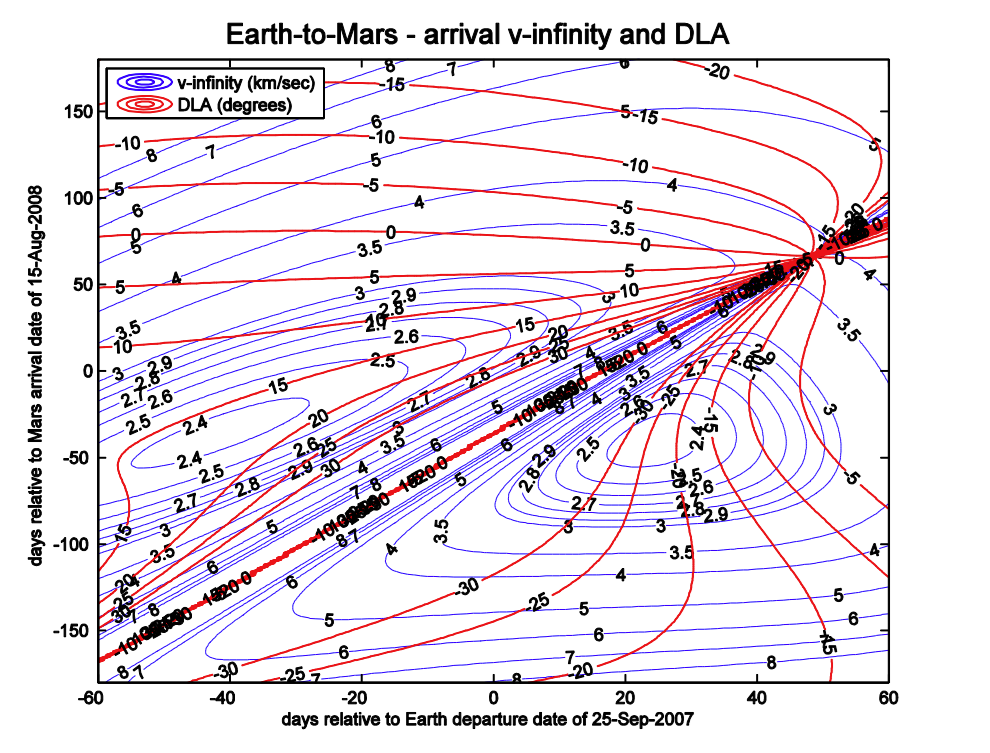
\includegraphics[width=0.4\textwidth]{porkchop_ejemplo.png}
    \captionof{figure}{Ejemplo de Porkchop plot.} \parencite{eagle2025}
\end{center}

\subsubsection{Método de Gibbs}
Una vez que se
han obtenido las estimaciones iniciales de $t_0$ y $t_1$ a partir del gráfico
Porkchop, se utiliza el Método de Gibbs para determinar la órbita
de la nave perseguidora. Gracias a esto, se reduce la cantidad de variables independientes
de seis a dos. Este concepto se explica más a profundidad en la sección de formulación del problema.

El método de Gibbs calcula la velocidad orbital de
la nave a partir de tres vectores de posición conocidos de la nave y
los dos objetivos \parencite{HE2010265}. A partir de los tres
vectores de posición $r_1$, $r_2$ y $r_3$, se calcula la velocidad de la nave
perseguidora en la órbita de intercepción con la siguiente fórmula:

\begin{equation}
    v_{3,tk} = \sqrt{\frac{\mu}{ND} \left( \frac{D \ast r_{3,tk}}{r_{3,tk}} + S \right)}
\end{equation}

Donde:
\begin{itemize}
    \item $v_{3,tk}$: vector de velocidad de la nave perseguidora en el tiempo $t_k$.
    \item $\mu$: constante gravitacional de la Tierra.
    \item N, D, y S\@: valores derivados del producto cruz entre los vectores de posición.
\end{itemize}

\subsubsection{Método de Newton-Raphson}
El Método de Newton-Raphson es un algoritmo iterativo utilizado para resolver sistemas de ecuaciones no lineales, y es esencial para refinar las soluciones obtenidas con los métodos anteriores.
En este caso, se utiliza para ajustar las variables $t_0$, $t_1$, $t_2$ y el vector de impulso $v$ hasta que se cumplan las condiciones de interceptación.

Fórmula de iteración:
\[
    x_{n+1} = x_n - J{(x_n)}^{-1} \ast F(x_n)
\]

Donde:
\begin{itemize}
    \item $x_n$ es el vector de valores actuales de las variables.
    \item $J$ es la matriz Jacobiana de las ecuaciones no lineales.
    \item $F(x_n)$ es el vector de funciones (las ecuaciones de las posiciones y tiempos de interceptación).
\end{itemize}

    \section{Formulación del problema}
El objetivo es interceptar dos objetos (naves, sálelites, etc) con un sólo impulso.
Para ello, planteamos seis variables independientes:

\begin{itemize}
    \item $t_0$: tiempo de impulso.
    \item $t_1$: tiempo de intercepción con el primer objetivo.
    \item $t_2$: tiempo de intercepción con el segundo objetivo.
    \item $\Delta{v}$: vector de impulso (contiene tres componentes).
\end{itemize}

Con el método de Gibbs, se calcula la velocidad de la nave perseguidora en los tiempos
$t_0$, $t_1$, y $t_2$. Con estos tres vectores, podemos determinar por completo la órbita
de interceptación. Luego, quedan 3 variables, en las siguientes ecuaciones:

\begin{equation}
    t_1 - t_0 = \frac{M_{3, t_1} - M_{3, t_0}}{n_3}
\end{equation}
\begin{equation}
    t_2 - t_0 = \frac{M_{3, t_2} - M_{3, t_0}}{n_3}
\end{equation}

Suponiendo que el tiempo inicial $t_i$ es conocido, y por tanto calculado $t_2$, y además despreciamos
el efecto de la perturbación J2, podemos expresar $t_2$ como una función de $t_1$ y $t_0$ \parencite{xia2021}.
Por lo tanto, el problema se reduce a dos variables independientes.

Con las ecuaciones (3) y (4), podemos armar el siguiente sistema de ecuaciones \parencite{xia2021}:

\begin{equation}
    \mathbf{F}(t_0, t_1) =
    \begin{Bmatrix}
        Q_1 \\ Q_2
    \end{Bmatrix}
    =
    \begin{Bmatrix}
        0 \\ 0
    \end{Bmatrix}
\end{equation}

donde
\begin{equation}
    \left\{
    \begin{aligned}
        Q_1 & = (t_1 - t_0) - \frac{M_{3, t_1} - M_{3, t_0}}{n_3} \\
        Q_2 & = (t_2 - t_0) - \frac{M_{3, t_2} - M_{3, t_0}}{n_3}
    \end{aligned}
    \right.
\end{equation}

Note que $t_0 < t_1 < t_2$.

Posteriormente, se estudiarán las variables $M_{j,t_k}$. Estos variables, que representan la anomalía,
media, se calculan con la ecuación de Kepler \parencite{xia2021}, y son críticas para el modelo matemático
ya que permiten calcular la posición de un objeto que se mueve en una de las tres órbitas, sobre todo la de interceptación.
    \section{Metodologia}
Esta sección describe detalladamente el procedimiento metodológico aplicado
para construir y resolver el modelo numérico de intercepción de dos objetivos
con un solo impulso, empleando métodos numéricos revisados y no revisados en
clase. El enfoque incluye la recolección y análisis de datos, el desarrollo del
algoritmo, la justificación metodológica y la identificación de limitaciones
del modelo.

\subsection{Recolección de datos}
Los datos utilizados para construir el modelo provienen de la Tabla 1 del
artículo de Xia et al. (2021), la cual define los elementos orbitales de tres
cuerpos: una nave perseguidora (S0) y dos objetivos (S1 y S2). Estos elementos
fueron introducidos en el modelo bajo el marco de un sistema de dos cuerpos,
tal como se planteó anteriormente.

Las herramientas y software utilizados se listan a continuación:

\begin{itemize}
    \item MATLAB, para la implementación computacional del modelo
    \item Funciones propias en MATLAB para la conversión de elementos orbitales,
          propagación de trayectorias, cálculo de anomalías y generación de Porkchop
          plots.
    \item Scripts adaptados para aplicar el método de Gibbs y resolver sistemas no
          lineales con Newton-Raphson
\end{itemize}

\subsection{Análisis de datos}
Se desarrolló un proceso iterativo compuesto por las siguientes etapas:

\subsubsection{Conversión de elementos orbitales}
A partir de los valores de periapsis $rp$ y apoapsis $ra$, se calculó el
semieje mayor $a$ y la excentricidad $e$ de acuerdo a las siguientes fórmulas:

\begin{itemize}
    \item $a = (rp + ra) / 2$
    \item $e = \frac{ra - rp}{ra + rp}$
\end{itemize}

\subsubsection{Transformación a vectores de estado}
Los elementos orbitales se convirtieron a vectores de posición y velocidad en
el sistema de coordenadas inerciales (ECI) usando funciones orbitales
conocidas.

\subsubsection{Generación de Porkchop plot}
Se exploró el espacio de tiempos de impulso $t_0$ e intercepción $t_1$ mediante
un Porkchop plot, evaluando la siguiente función para cada combinación:

$P = \left| t_1 - t_0 - \frac{M_{3, t_1} - M_{3, t_0}}{n_3} \right| + \left| t_2 - t_0 - \frac{M_{3, t_2} - M_{3, t_0}}{n_3} \right|$

Esto permitió seleccionar pares iniciales con valores mínimos de P como
candidatos para el método de Newton-Raphson \parencite{Wang2025}.

\subsubsection{Cálculo de t\textsubscript{2}}
A partir de los parámetros de $S_2$, se estimó $t_2$ utilizando la propagación
de la anomalía media para el segundo objetivo:

$t_2 = \frac{M_{2, t_2} - M_{2,t_i}}{n_2}$

\subsubsection{Método de Gibbs}
Con los vectores de posición $r_0$, $r_1$, y $r_2$, se utilizó el método de
Gibbs para calcular el vector de velocidad orbital de la nave perseguidora:

$v_{3, t_k} = \sqrt{\frac{\mu}{ND}} \left( \frac{\textbf{D} \times \textbf{r}_{3, t_k}}{r_{3, t_k}} + \textbf{S} \right)$

\subsubsection{Formulación de sistema no lineal}
Se planteó el siguiente sistema con las ecuaciones (3) y (4)

\begin{equation}
    \begin{cases}
        Q_1 = t_1 - t_0 = \dfrac{M_{3, t_1} - M_{3, t_0}}{n_3} \\
        Q_2 = t_2 - t_0 = \dfrac{M_{3, t_2} - M_{3, t_0}}{n_3}
    \end{cases}
\end{equation}

\subsubsection{Resolución con Newton-Raphson}
Se resolvió el sistema anterior usando el método de Newton-Raphson con
derivadas parciales analíticas en las variables $t_0$ y $t_1$ con una
tolerancia de $10e^{-5}$.

\subsubsection{Validación de resultados}
Se verificó la convergencia numérica y se graficaron las trayectorias de las
tres naves, confirmando intercepciones visuales con $S_1$ y $S_2$.

\subsection{Algoritmo}

A continuación, se presenta la serie de pasos a seguir para aplicar el método
al problema formulado:

\begin{enumerate}
    \item Cargar datos orbitales de S0, S1 y S2.
    \item Calcular $a$ y $e$ para cada cuerpo.
    \item Transformar elementos orbitales a vectores $(\mathbf{r}, \mathbf{v})$.
    \item Crear matriz de tiempos $t_0$, $t_1$ $\rightarrow$ Porkchop plot:
          \begin{enumerate}
              \item Calcular $t_2$ a partir de $M_2$ y $n_2$.
              \item Calcular error $P(t_0, t_1)$.
          \end{enumerate}
    \item Seleccionar pares con menor $P$ como estimaciones iniciales.
    \item Para cada par seleccionado:
          \begin{enumerate}
              \item Calcular $\mathbf{r}_0$, $\mathbf{r}_1$, $\mathbf{r}_2$.
              \item Calcular $\mathbf{v}$ mediante método de Gibbs.
              \item Determinar $M_3$ en $t_0$, $t_1$, $t_2$ y $n_3$.
              \item Resolver sistema no lineal con Newton-Raphson.
              \item Evaluar convergencia y guardar solución.
          \end{enumerate}
    \item Visualizar trayectorias y validar intercepciones.
\end{enumerate}

\subsection{Diagrama de flujo}

\begin{figure}[H]
    \centering
    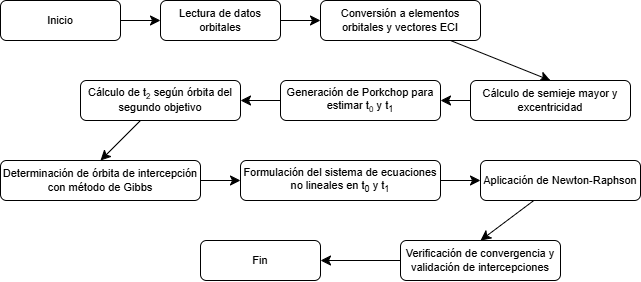
\includegraphics[width=0.9\textwidth]{flowchart.png}
    \caption{Diagrama de flujo del algoritmo propuesto.}
    \label{fig:flowchart}
\end{figure}

\newpage

\subsection{Justificación de método}
\begin{itemize}
    \item \textbf{Newton-Raphson}: Su velocidad de convergencia y precisión lo hacen adecuado para resolver sistemas no lineales con pocas variables, como el planteado.
    \item \textbf{Gibbs}: Permite estimar la velocidad orbital de una nave a partir de tres vectores de posición sin necesidad de integrar ecuaciones diferenciales.
    \item \textbf{Porkchop plot}: Nos permite explorar las combinaciones de tiempos de impulso e intercepción, optimizando la elección de valores iniciales.
\end{itemize}

\subsection{Limitaciones del enfoque}

\begin{enumerate}
    \item El modelo no considera perturbaciones como el término J2, lo que puede generar
          desviaciones en escenarios reales prolongados, o órbitas en las que el cuerpo
          central tiene una topología altamente irregular.

    \item La velocidad de convergencia de Newton-Raphson depende de las condiciones
          iniciales; elecciones pobres pueden generar fallas.

    \item Por otro lado, Gibbs requiere que los vectores de posición no sean colineales,
          lo que puede limitar su uso en situaciones particulares.
\end{enumerate}


    \section{Resultados}

Al realizar un Porkchop plot con la data obtenida de la tabla 1
\parencite{xia2021}, obtuvimos el siguiente resultado:

\begin{center}
    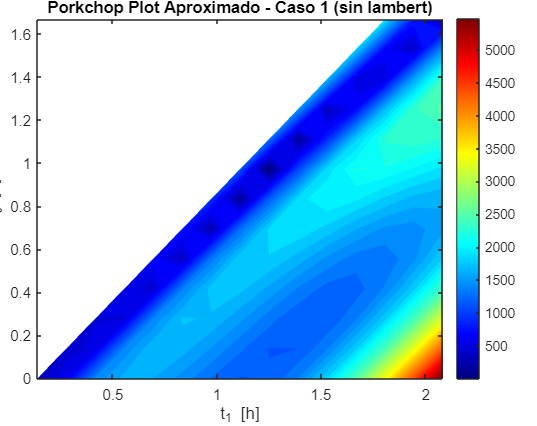
\includegraphics[width=0.4\textwidth]{porkchop_emma.jpg}
    \captionof{figure}{Porkchop resultante}
\end{center}

Las franjas azules indican mínimos, los cuales muestran una posible ventana de
impulso para interceptar a los dos objetos.
    \section{Discusión}

    \section{Conclusiones}

En este estudio se logró simular el escenario de interceptación orbital doble
con un solo impulso, correspondiente al caso 1 que sigue la ruta $S_0
    \rightarrow S_1 \rightarrow S_2$, mediante la generación de un Porkchop plot y
la implementación del método de Gibbs.

El Porkchop nos permitió ver las regiones temporales donde se facilita realiza
la transferencia orbital con bajo error temporal. Esto se puede evidenciar por
la aparición de una franja azul, la cual representa los pares temporales de
$t_0$ y $t_1$ que mejor se ajustan a una buena trayectoria. Este resultado
confirma que existen combinaciones viables de eventos temporales para realizar
una doble interceptación bajo el modelo de dos cuerpos, validando uno de los
principales objetivos del trabajo.

Además, se utilizó el método de Gibbs, el cual estima el vector de velocidad en
el punto intermedio de intersección $S_1$, a partir de las posiciones dadas con
los elementos orbitales. Esta estimación resulta coherente con los valores
esperados para orbitales de este tipo.

Los resultados obtenidos de Porkchop y el método de Gibbs ayudan a una
metodología efectiva para la planificación de trayectoria con múltiples
objetivos.
    \section{Recomendaciones}
\begin{itemize}
    \item \textbf{Incorporar perturbaciones en futuras versiones del modelo}: Para aumentar la
          precisión, se recomienda incluir efectos como el término J2, resistencia
          atmosférica o perturbaciones solares en simulaciones futuras, especialmente en
          misiones prolongadas o de mayor sensibilidad dinámica.
    \item \textbf{Extender el modelo a misiones interplanetarias o multiobjetivo}: El modelo puede adaptarse a misiones más complejas que involucren múltiples intercepciones en diferentes planos orbitales o destinos fuera de la órbita terrestre.
    \item \textbf{Aplicar el modelo en misiones de defensa espacial o inspección satelital}: Dada su capacidad para planificar trayectorias eficientes con mínimo impulso, el modelo es útil en misiones de interceptación de satélites, maniobras evasivas o misiones de servicio y desorbitación.
    \item \textbf{Comparar con otros métodos de resolución no lineal}: Se recomienda explorar métodos alternativos como gradiente conjugado, Levenberg-Marquardt o métodos metaheurísticos (ej. algoritmos genéticos) para resolver el sistema de ecuaciones no lineales, comparando tiempos de convergencia y estabilidad.
    \item \textbf{Desarrollar una interfaz gráfica interactiva en MATLAB}: Implementar una interfaz que permita visualizar Porkchop plots y trayectorias de forma dinámica facilitaría su uso didáctico o su aplicación por parte de operadores de misión.
    \item \textbf{Validar el modelo con escenarios reales de misiones espaciales}: Se sugiere aplicar el modelo a trayectorias reales (por ejemplo, misiones de la NASA o SpaceX) para validar su precisión y utilidad práctica en planificación de maniobras reales.
\end{itemize}

\end{multicols}
\newpage
\printbibliography[title={Referencias}]

\appendix
\section*{Anexo}
El código de MATLAB utilizado está disponible en el siguiente repositorio de GitHub:

\begin{itemize}
    \item \url{https://github.com/DanielCasquino/metnum_g9}
\end{itemize}

\end{document}